\documentclass{article}
\usepackage[utf8]{inputenc}
\usepackage[spanish]{babel}
\usepackage{graphicx}
\usepackage{amsfonts}

\begin{document}
%Portada
  \begin{figure}[lt]
    \includegraphics[width=0.3\textwidth]{ull.eps}
  \end{figure}
  \title{Integración Del Trapecio}
  \author{Tiffany López Nicholson \\ Miriam Martín Jacinto \\ Sergio Vega García}
  \date{\today}
  \maketitle

  \begin{abstract}
    \begin{center}
       A continuación se presentará como se ha implementado con python un algoritmo capaz de resolver la integral definida $\int_{1}^{6} \frac{1}{1+e^x}$
    \end{center}
  \end{abstract}
  \pagebreak

%%%%%%%%%%%%%%%%%%%%%

  \tableofcontents
  \pagebreak
  
%%%%%%%%%%%%%%%%%%%%%
  
  \section{Motivaciones y objetivos}
    \begin{itemize}
      \item Objetivo principal: Implementar con Python la integración del trapecio para f(x)
      \item Objetivo específico: Realizar un algoritmo capaz de resolver la integración del trapecio para $ f(x) = \frac{1}{1 + e^{x}}$, x E [1, 6],
    \end{itemize}
    \subsection{Seccion uno} % MIRAR SI VAMOS A INTRODUCIR
    \subsection{Seccion dos} % ALGO MÁS AQUÍ, O BORRARLO
  \pagebreak

%%%%%%%%%%%%%%%%%%%%%

  \section{Fundamentos teóricos}
    La regla del trapecio es un método de integración numérica que se basa en aproximar el valor de la integral definida de $f(x)$ por el de la función lineal que pasa a través de ésta, formándose una figura: un trapecio. Para obtener esta aproximación, debemos calcular el área de los trapecios.
    
    \begin{figure}[h]
      \begin{center}
	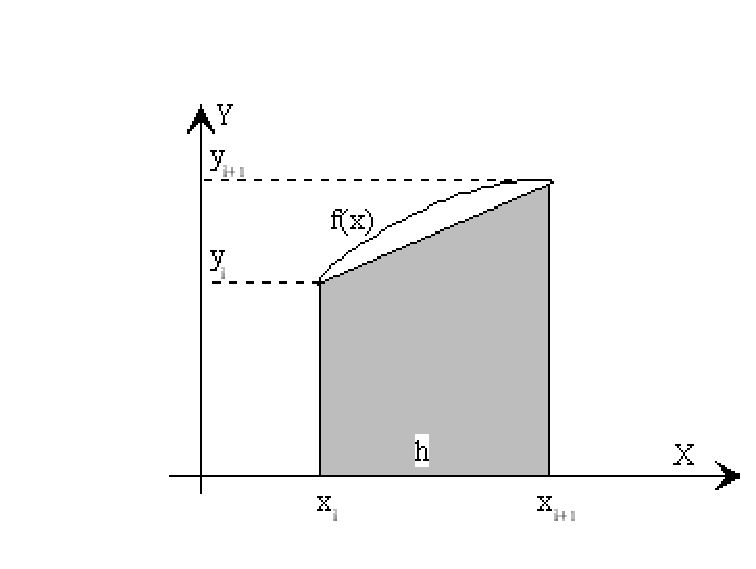
\includegraphics[scale=0.5]{areadeltrapecio.eps}
	\caption{Ejemplo}
      \end{center}
    \end{figure}

      Para justificar este método, deberemos ''aproximar'' de una buena manera nuestra función $f(x)$. Esto lo haremos gracias a la \textit{interpolación polinomial}.

    \subsection{Interpolación polinomial.}
      La interpolación polinomial nos dice que para hacer una ''buena aproximación''de $f(x)$, que querremos integrar, por otra función $g(x)$, en los puntos $x_{i}$ (con $i = 1, 2, 3, ..., n$); o lo que es lo mismo, $\int_{x_{1}}^{x_{n}}f(x)dx \approx \int_{x_{1}}^{x_{n}}g(x)dx$, $\forall x_{i}, con i = 1, 2, 3, ..., n$. Estas dos funciones deben ser continuas en el intervalo $[x_{1}, x_{n}]$.\\
%%NO HACE FALTA PONER CORCHETES PARA ELEVADOS O ÍNDICES SI SOLO ES UN DATO
%%PUEDES AHORRAR TIEMPO SI LOS EVITAS.
      Pero el problema que se presenta es como buscar estas funciones. Hay varios teoremas que nos ayudan a resolverlo, como el \textit{teorema aproximación de Weierstrass} o el \textit{polinomio de interpolación de Lagrange}.
      
    \subsection{Integración del trapecio}

      Para la utilización del método del trapecio partimos de una función, la cual dividiremos en n trozos iguales. Cuanto mayor sea el número de particiones, mayor precisión tendrá el método.\\

  	\begin{center}
         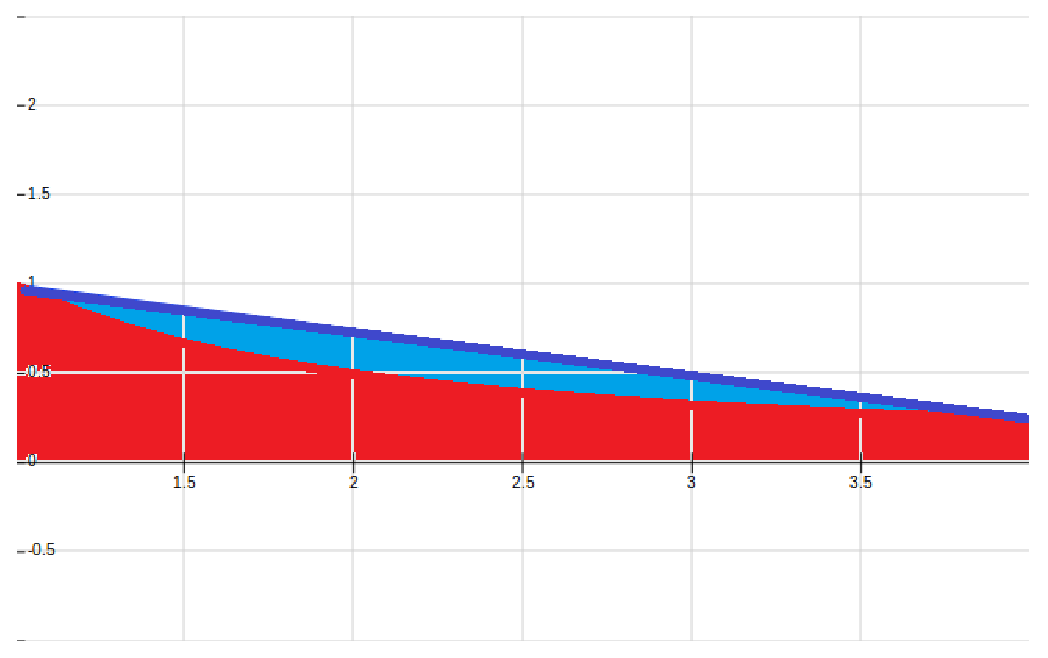
\includegraphics[width=0.48\textwidth]{img2.eps}
	 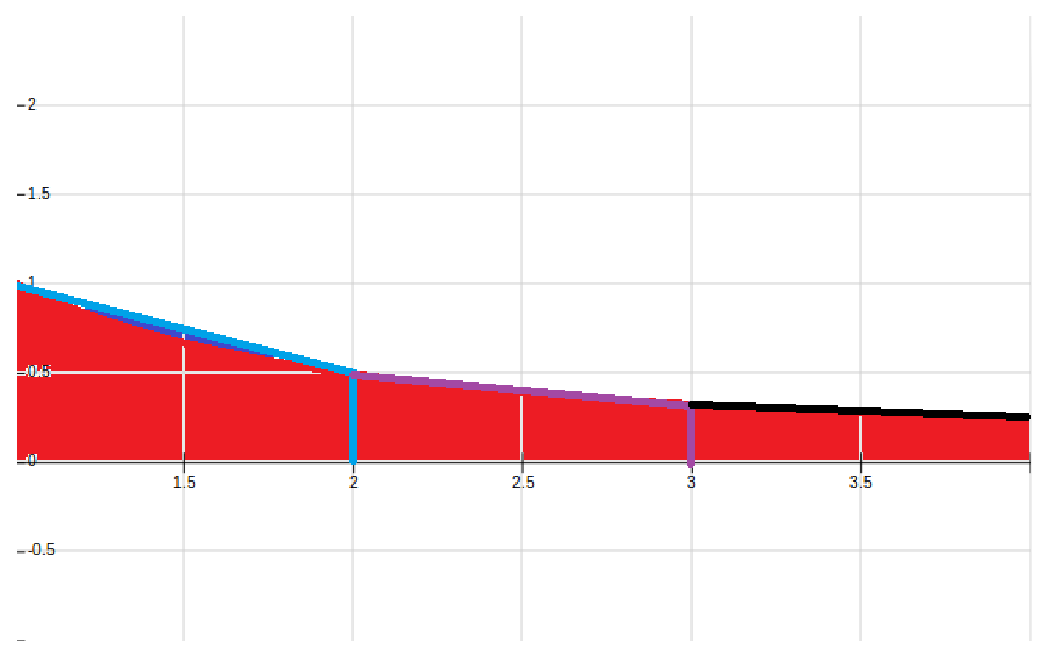
\includegraphics[width=0.48\textwidth]{img3.eps}
        \end{center}


      Se puede apreciar que el área tomada por exceso, es decir, la que supera a la función, o la tomada por defecto, la cual no llega a la función, se reduce según aumenta el número de particiones. \\
      \\

      La función general es: 
        
      \begin{center}
   
        $\int_{a}^{b}f(x)dx \approx \frac{h}{2}[f(a)-2f(a+h)+2f(a+2h)+...+f(b)]$

      \end{center}
 
      Donde $h=\frac{b-a}{n}$ y n es el número de divisiones.\\

      La expresión anterior también se puede escribir como:

      \begin{center}

        $\int_{a}^{b}f(x)dx \approx \frac{b-a}{n}(\frac{f(a)+f(b)}{2}+\sum\limits_{k=1}^{n-1}f(a+k\frac{b-a}{n}))$
      \end{center}

    \subsection{Integración del trapecio aplicado}
      
    La ecuación específica del proyecto es $f(x)\frac{1}{1+e^x}$, cuya representación gráfica es la siguiente:
     
     \begin{figure}[h]
      \begin{center}
         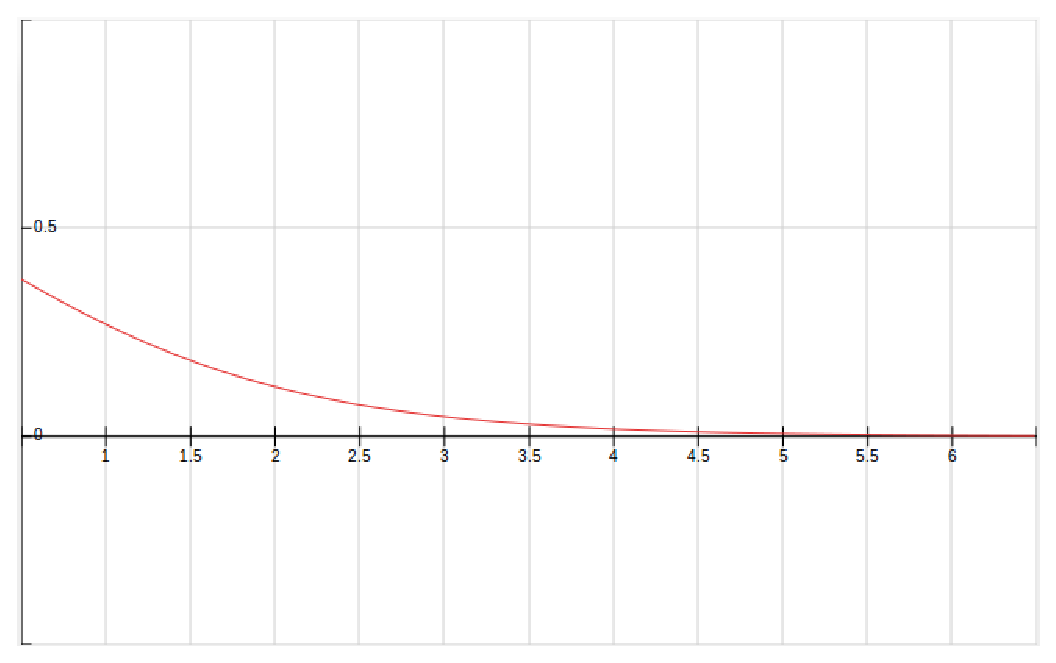
\includegraphics[width=0.7\textwidth]{img4.eps}
      \end{center}
     \end{figure}

      El intervalo de la integral es [1,6]. Existe función en todos los puntos, por lo que también existe la integral. Al igual que en el caso anterior, por existir una curva, habría que realizar varias particiones para conseguir un resultado preciso.

   \pagebreak

%%%%%%%%%%%%%%%%%%%%%%%%%%%%%%%%%%

%BOCETOOOOOOOOOOOO

   \section{Procedimiento experimental}
   Para poder realizar la integración del trapecio primero necesitabamos analizar los datos iniciales.
   \begin{itemize}
    \item La función $f(x)=\frac{1}{1+e^x}$ estaba definida en el intervalo [1,6].
    \item La función definida en [1,6] existe en $\mathbb{R}$, numeros reales, por tanto se puede integrar.
    \item En la fórmula de la integración del trapecio intervienen bastantes variables.
   \end{itemize}
   Con estos datos a priori se pueden sacar dos conclusiones.
     \begin{enumerate}
       \item Realizar la integración por la regla del trapecio manualmente es muy tedioso.
       \item Se necesita implementar un programa en python para agilizar la tarea.
     \end{enumerate}

   Se ha creado en python un programa que permita elegir el número de particiones y así comparar resultados. La utilidad principal sería comprobar que cuantas más particiones se realicen, más precisa es la integración.
    
    \subsection{Descripción de los experimentos}

   Se ha implementado un programa en python capaz de realizar la regla del trapecio, y que podamos elegir particiones mínimas y máximas. Al ejecutarlo e introducir los datos nos va mostrando los resultados de cada partición.\\

   Se han comprobado algunas particiones manualmente para comprobar que realmente el programa está funcionando correctamente.\\

   Se ha ejecutado dos veces el bucle con las siguientes caracteristicas:
 
   \begin{enumerate}
     \item De 1 a 10 particiones, con intervalo de 1 unidad.
     \item De 1 a 101 particiones, con intervalo de 10 unidades.
   \end{enumerate}

    \subsection{Descripción del material}

      \begin{itemize}
        \item S.O. original: Windows
        \item S.O. utilizado: Linux
        \item Procesador: 2.2 GHz
        \item Velocidad: 1200.000 MHz
        \item RAM: 4014144 kB
        \item Programa: Python
      \end{itemize}

    \subsection{Resultados obtenidos}

    \subsection{Análisis de resultados}

   \pagebreak

%FIN BOCETO
%%%%%%%%%%%%%%%%%%%%%%%%%%%%%%%%%%
\end{document}
